En esta sección se demuestra el potencial de la herramienta con algunos ejemplos de su comportamiento. Validando  sus mejoras funcionales con respecto a la versión de Scratch4Robots de la que partimos. Siguiendo el ciclo de vida de la aplicación aplicación y explicando el proceso que lleva a la consecución de los objetivo.\\

Además de los comportamientos mostrados en este apartado, se ha creado una batería de pruebas con las que ver un ejemplo de comportamiento de cada uno de nuestros bloques. Estas pruebas son proyectos Scratch que el usuario puede cargar en el entorno de Scratch y usar como punto de partida para sus próximos proyectos.

\section{Evitar obstáculos con Turtlebot}
\label{sec:evitar-obstaculos}

En este ejemplo hacemos uso de un robot sobre ruedas, para ser más exactos, de un Turtlebot. Para ejecutar las pruebas utilizamos Gazebo como simulador, cargando un entorno con obstáculos repartidos como se aprecia en la figura 6.2.\\

El objetivo directo de este experimento es la programación de un robot Turtlebot, capaz de evitar obstáculos de forma autónoma, con la ayuda de un sensor láser incorporado en su parte frontal. Esto se consigue usando únicamente la lógica de la que disponemos en Scratch junto con la extensión que aporta nuestra aplicación Scratch4Robots.\\

En estos comportamientos de ejemplo se puede apreciar el poder didáctico de la herramienta. Su simplicidad y sencillez hacen de ella perfecta para la enseñanza a personas con pocos conocimientos técnicos.\\

Además este ejemplo se puede ver día a día con las famosas aspiradoras autónomas (iRobot Roomba), aplicación directa que podría tener la aplicación fuera del ámbito didáctico.\\

En primer lugar y con ayuda de los bloques visuales, se desarrolla la aplicación en el editor Scratch. Una vez tenemos nuestro proyecto acabado y guardado, con la herramienta Scratch4Robots, ya instalada en el equipo y mediante el uso de un solo comando se realiza la traducción del proyecto.\\

\begin{figure}[H]
    \centering
    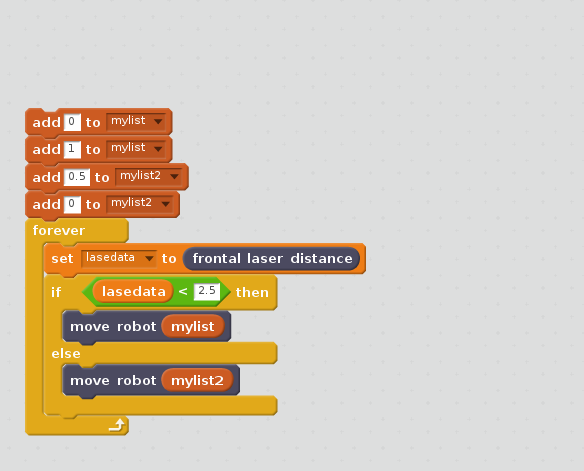
\includegraphics[scale=0.60]{img/robot-obstaculos-scratch.PNG}
  	\caption{programación en Scratch del Turtlebot}
  	\label{fig:turtlebot}
\end{figure}
Esta simpleza en la ejecución se consigue mediante las funcionalidades que aporta ROS para la ejecución de nodos, esto se consigue tras la labor de integración realizada. El comando a ejecutar sería:

\begin{lstlisting}[language=json,firstnumber=1]
~$ rosrun scratch4robots scratch2python myscratchaproyect.sb2
\end{lstlisting}


Explicando un poco el comando anterior, \textit{rosrun} es el comando que nos aporta ROS, capaz de ejecutar nodos de un paquete ROS, \textit{scratch4robots} es el paquete ya instalado en la máquina, \textit{scratch2python} el nodo interno de la aplicación encargada de la traducción a Python, y por último \textit{myscratchaproyect.sb2} es el proyecto Scratch que se quiere traducir. Se aprecia a continuación el código ya traducido a Python que será incrustado en el nodo ROS para su ejecución.

\begin{lstlisting}[language=python,firstnumber=1]
        mylist = []
        mylist2 = []
		# Agrega velocidades que realizan el giro del Turtlebot
        mylist.append('0')
        mylist.append('1')
        # Agrega velocidades que hacen que el Turtlebot avance
        mylist2.append('0.5')
        mylist2.append('0')
        while True:
            lasedata = robot.get_laser_distance()
            if lasedata < 2.5:
                robot.move_vector(mylist)
            else:
                robot.move_vector(mylist2)
                
\end{lstlisting}

Tras la traducción se obtiene un nodo ROS con el mismo nombre que tenía el proyecto Scratch, completamente preparado para su ejecución sobre el robot Turtlebot, únicamente con la dependencia de un fichero de configuración que describiremos a continuación:
\begin{lstlisting}[language=json,firstnumber=1]
robot:
  Motors:
    Topic: "/mobile_base/commands/velocity"
    Name: robotMotors
  Laser:
    Topic: "/scan"
    Name: robotLaser
  Pose3D:
    Topic: "/odom"
    Name: robotPose3d
  Camera1:
    Format: RGB8
    Topic: "/cameraL/image_raw"
    Name: robotCamera1
  NodeName: robot
\end{lstlisting}
En este fichero se definen los distintos actuadores y sensores que necesitará nuestro nodo, además por cada sensor se define el Tópico al que el nodo se subscribe para enviar y recoger los datos que necesita del robot. En este caso darle especial importancia a la obtención de los datos del sensor láser, protagonista de nuestro ejemplo.

Con todo esto preparado solo faltaría ejecutar nuestro nodo sobre la simulación para ver los resultados que podemos apreciar en el siguente detalle\footnote{\url{https://www.youtube.com/watch?v=SCd2h3mP0-k}}.

\begin{figure}[H]
    \centering
    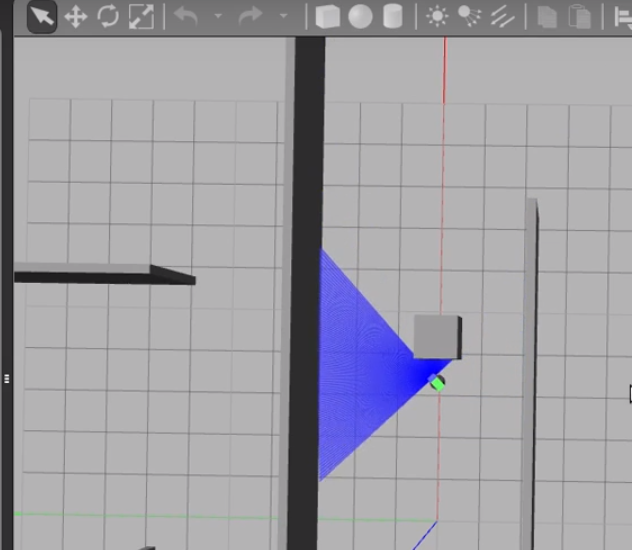
\includegraphics[scale=0.75]{img/robot-example.PNG}
  	\caption{Comportamiento de evitación de obstáculos en Turtlebot}
  	\label{turtlebot-scr}
\end{figure}


De esta forma, se cumple con el objetivo de esta validación. 


\section{Persecución entre drones}
\label{sec:persecucion-drones}

En este ejemplo por el contrario, como robot final se usa un dron, mucho más interesante desde el punto de vista práctico, aunque igual de interesante desde el punto de vista didáctico. Al igual que con la prueba anterior se utiliza Gazebo como motor de simulación.\\

El ciclo de vida es el mismo que el que hemos seguido para la ejecución del robot. Primero se genera el proyecto en Scratch, el cual se muestra en la siguiente imagen:\\

\begin{figure}[H]
    \centering
    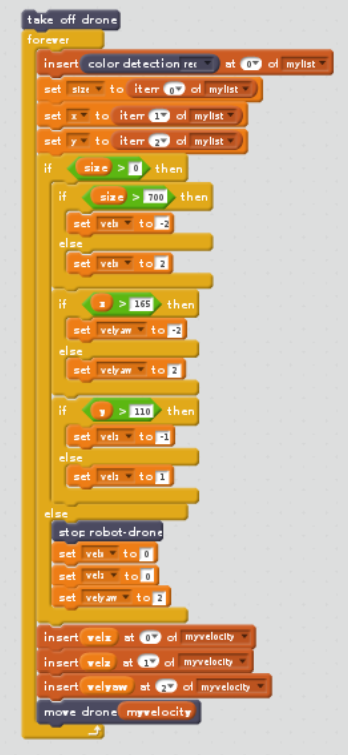
\includegraphics[scale=0.75]{img/cat-drone-scratch.PNG}
  	\caption{Programación en Scratch del drone perseguidor}
  	\label{fig:drone-perse}
\end{figure}

Mediante las funcionalidades que aporta ROS para el lanzamiento de aplicaciones bajo un solo comando ejecuta la traducción, obteniendo nuestro nodo programado en Python del mismo nombre que el proyecto Scratch. Se muestra el detalle de la traducción de este proyecto, la cual se integrará en el nodo final ROS como se describe en apartados anteriores.

\begin{lstlisting}[language=python,firstnumber=1]
 		mylist = [] 
 		myvelocity = []
        robot.take_off()
        while True:
            mylist.insert(0, robot.color_detection('red'))
            size = mylist[0][0]
            x = mylist[0][1]
            y = mylist[0][2]
            if size > 0: 		 # Tras detectar el objetivo, estima velocidades
                if size > 700:
                    velx = '-2'
                else:
                    velx = '2'
                if x > 165:
                    velyaw = '-2'
                else:
                    velyaw = '2'               
                if y > 110:
                    velz = '-1'
                else:
                    velz = '1'               
            else:			# Gira sobre si mismo buscando el objetivo
                robot.stop()
                velx = '0'
                velz = '0'
                velyaw = '2'            
            myvelocity.insert(0, velx)
            myvelocity.insert(1, velz)
            myvelocity.insert(2, velyaw)
            robot.move_vector(myvelocity)
\end{lstlisting}

Y por último, ya con el nodo generado, agregando la configuración pertinente estará todo listo para su ejecución.

\begin{lstlisting}[language=json,firstnumber=1]
drone:
  Camera:
    Topic: "/solo/cam_frontal/image_raw"
    Name: UAVViewerCamera    
  Pose3D:
    Topic: "/mavros/local_position/odom"
    Name: UAVViewerPose3d
  CMDVel:
    Topic: "/mavros/setpoint_velocity/cmd_vel"
    Name: UAVViewerCMDVel    
  Navdata:
    Topic: "/IntrorobROS/Navdata"
    Name: UAVViewerNavdata 
  Extra:
    TopicArming: "mavros/cmd/arming"
    TopicLand: "mavros/cmd/land"
    TopicSetMode: "mavros/set_mode"
    TopicVel: "/mavros/setpoint_velocity/cmd_vel"
    Name: UAVViewerExtra
NodeName: drone
\end{lstlisting}
Tras ejecutar el nodo junto con el fichero de configuración, se obtiene el resultado deseado. Algo tan complejo como una persecución entre dos drones, totalmente programado en un lenguaje tan simple como Scratch, y esto, es solo una prueba del potencial de esta herramienta.\\

En la siguiente secuencia se aprecia el comportamiento deseado.

\begin{figure}[H]
    \centering
    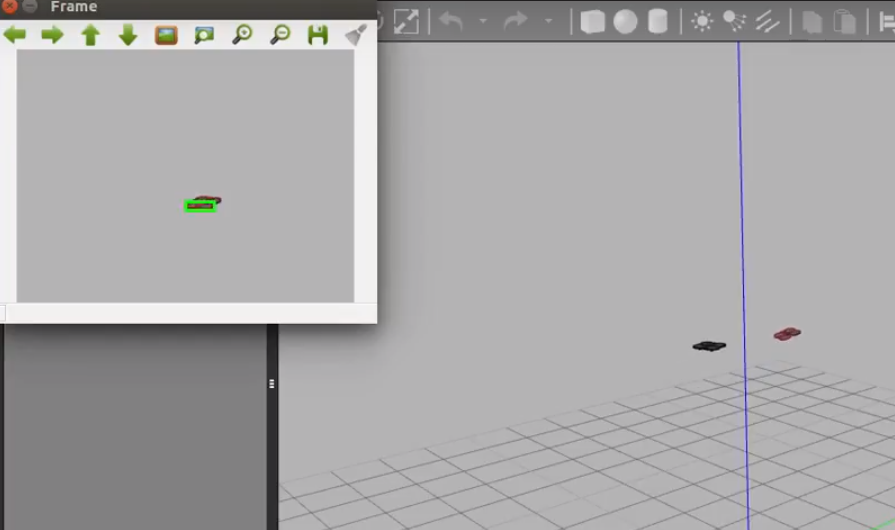
\includegraphics[scale=0.50]{img/cat1.PNG}
  	\caption{secuencia de ejecución del drone perseguidor}
  	\label{fig:drone-pers}
\end{figure}
\begin{figure}[H]
    \centering
    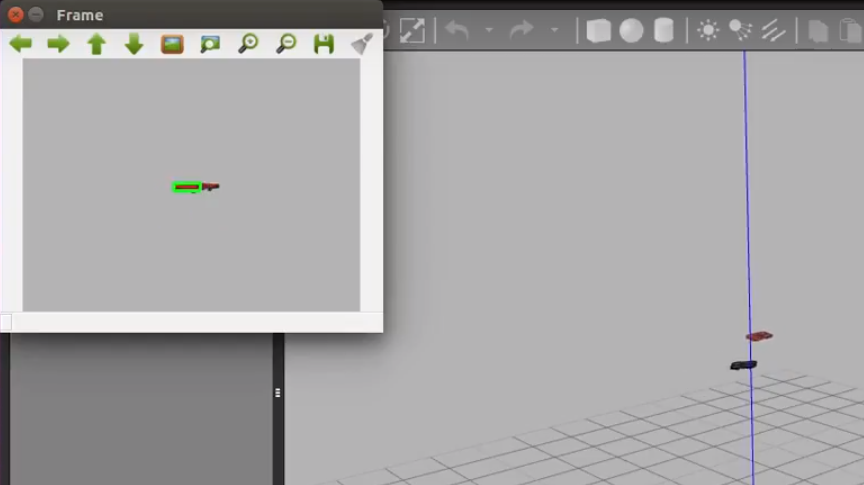
\includegraphics[scale=0.50]{img/cat2.PNG}
  	\caption{secuencia de ejecución del drone perseguidor}
  	\label{fig:drone-pers}
\end{figure}
\begin{figure}[H]
    \centering
    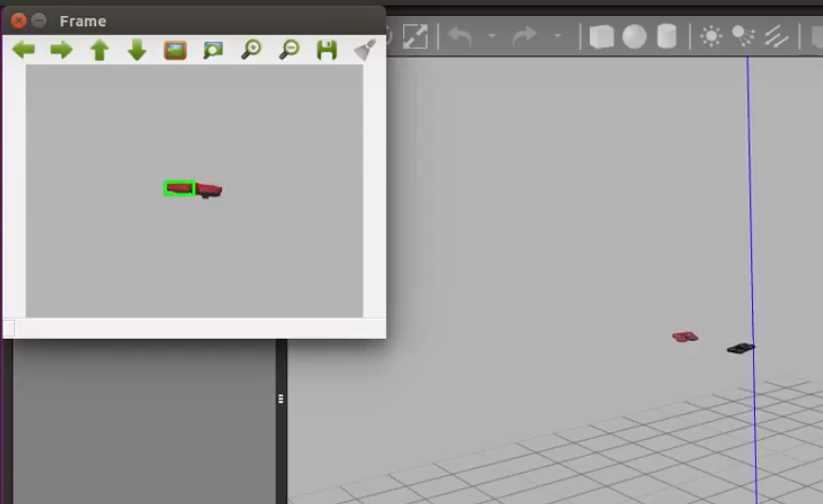
\includegraphics[scale=0.50]{img/cat3.PNG}
  	\caption{secuencia de ejecución del drone perseguidor}
  	\label{fig:drone-pers}
\end{figure}


Con estos ejemplos se recorre el ciclo de vida de nuestra herramienta, explicando su funcionamiento, además de validar experimentalmente todas las mejoras en el funcionamiento de Scratch4Robots 2.0. Las mejoras en la ejecución de la herramienta mediante simples comandos, sin necesidad de indagar en el código fuente. Y completo funcionamiento de la herramienta, con comunicaciones puramente ROS. 

